% PINN architecture schematic for the inverse Burgers Tesseract.
% Compile:   pdflatex pinn_architecture.tex
% Rasterize: pdftoppm -png -r 300 pinn_architecture.pdf raw \
%            && magick raw-1.png -trim +repage pinn_architecture.png
\documentclass{article}
\usepackage[paperwidth=23cm, paperheight=9cm, margin=3mm]{geometry}
\usepackage{tikz}
\usepackage{amsmath}
\usepackage{amssymb}
\usepackage{bm}
\usetikzlibrary{positioning, arrows.meta, backgrounds, fit, calc}
\pagestyle{empty}

% Shared brand palette (refined light)
\definecolor{cInput}{HTML}{44566C}    % slate
\definecolor{cFourier}{HTML}{3D3D9E}  % indigo
\definecolor{cHidden}{HTML}{0E6E6E}   % deep teal
\definecolor{cOut}{HTML}{9E2B3A}      % crimson
\definecolor{cDeriv}{HTML}{B5760A}    % amber
\definecolor{cEdge}{HTML}{9AA5AD}     % muted gray

\begin{document}
\noindent
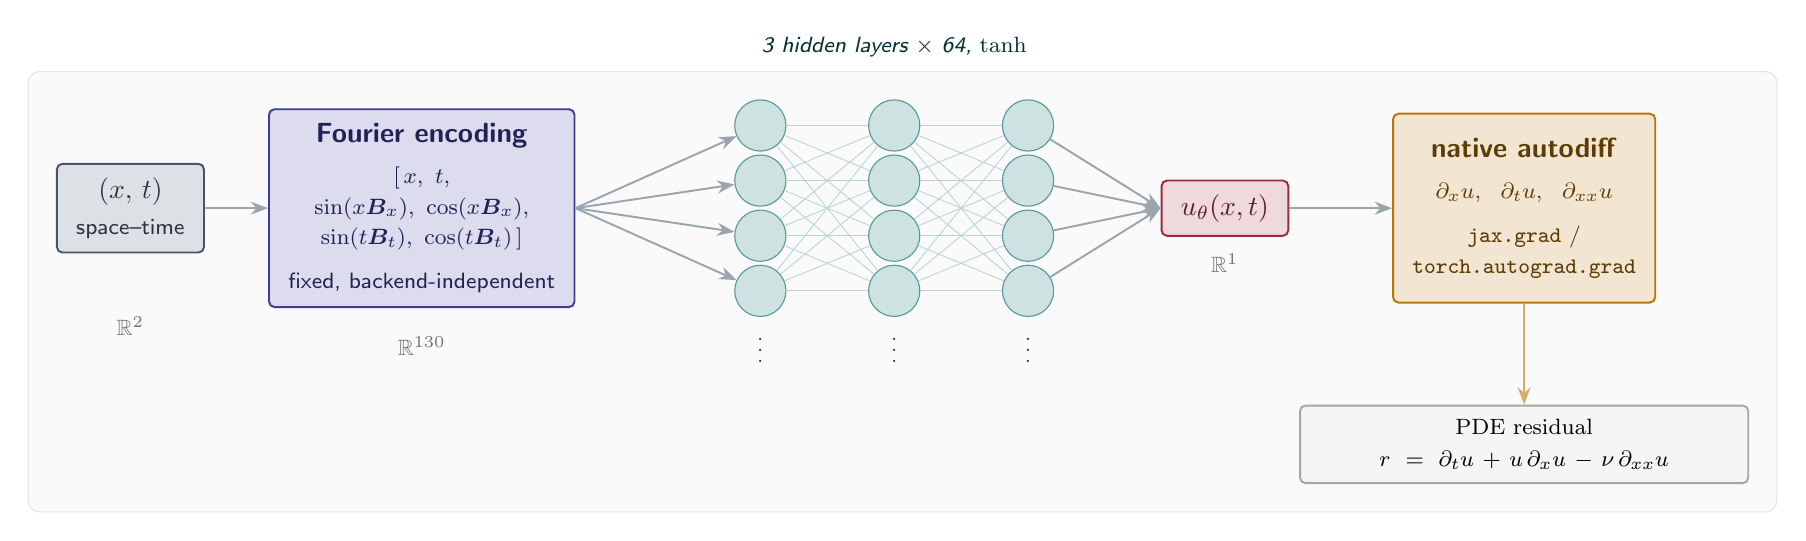
\begin{tikzpicture}[
  font=\sffamily,
  >={Stealth[length=2.2mm]},
  block/.style={rounded corners=2pt, draw=black!55, line width=0.7pt,
                inner xsep=7pt, inner ysep=5pt, align=center},
  neuron/.style={circle, draw=cHidden!70, fill=cHidden!20, line width=0.4pt,
                 minimum size=6.5mm},
  lab/.style={font=\sffamily\footnotesize\itshape, text=black!55},
  flow/.style={->, draw=cEdge, line width=0.7pt},
]

% ---- Input coordinates -------------------------------------------------
\node[block, fill=cInput!18, draw=cInput, text=cInput!60!black] (in) at (0,0)
  {$(x,\,t)$\\[1pt]\footnotesize space--time};

% ---- Fixed Fourier feature encoding -----------------------------------
\node[block, fill=cFourier!18, draw=cFourier, text=cFourier!55!black,
      minimum height=24mm] (fourier) at (3.7,0)
  {\textbf{Fourier encoding}\\[3pt]
   \footnotesize$[\,x,\ t,$\\[-1pt]
   \footnotesize$\sin(x\bm{B}_x),\ \cos(x\bm{B}_x),$\\[-1pt]
   \footnotesize$\sin(t\bm{B}_t),\ \cos(t\bm{B}_t)\,]$\\[4pt]
   \footnotesize fixed, backend-independent};

% ---- MLP hidden layers (3 x 64, tanh) ---------------------------------
\foreach \i in {1,2,3} {
  \pgfmathsetmacro{\xpos}{8.0 + 1.7*(\i-1)}
  \begin{scope}[shift={(\xpos,0)}]
    \foreach \y [count=\j] in {1.05,0.35,-0.35,-1.05} {
      \node[neuron] (h\i\j) at (0,\y) {};
    }
    \node[font=\scriptsize, text=cHidden!60!black] at (0,-1.7) (h\i d) {$\vdots$};
  \end{scope}
}
\node[lab, text=cHidden!45!black] at (9.7,2.05)
  {3 hidden layers $\times$ 64, $\tanh$};

% sparse inter-layer edges for readability
\foreach \a in {1,2,3,4} {
  \foreach \b in {1,2,3,4} {
    \draw[draw=cHidden!30, line width=0.3pt] (h1\a) -- (h2\b);
    \draw[draw=cHidden!30, line width=0.3pt] (h2\a) -- (h3\b);
  }
}

% ---- Network output u ---------------------------------------------------
\node[block, fill=cOut!18, draw=cOut, text=cOut!58!black] (u) at (13.9,0)
  {$u_\theta(x,t)$};

% ---- Native autodiff derivatives ---------------------------------------
\node[block, fill=cDeriv!18, draw=cDeriv, text=cDeriv!52!black,
      minimum height=24mm] (deriv) at (17.7,0)
  {\textbf{native autodiff}\\[3pt]
   \footnotesize$\partial_x u,\ \ \partial_t u,\ \ \partial_{xx} u$\\[4pt]
   \footnotesize\texttt{jax.grad} /\\[-1pt]
   \footnotesize\texttt{torch.autograd.grad}};

% ---- Connections --------------------------------------------------------
\draw[flow] (in) -- (fourier);
\foreach \j in {1,2,3,4} { \draw[flow] (fourier.east) -- (h1\j); }
\foreach \j in {1,2,3,4} { \draw[flow] (h3\j) -- (u.west); }
\draw[flow] (u) -- (deriv);

% ---- Dimension annotations ---------------------------------------------
\node[lab] at (0,-1.5) {$\mathbb{R}^2$};
\node[lab] at (3.7,-1.75) {$\mathbb{R}^{130}$};
\node[lab] at (13.9,-0.7) {$\mathbb{R}^1$};

% ---- PDE residual readout ----------------------------------------------
\node[block, draw=black!35, fill=black!4, font=\footnotesize, text width=52mm]
      (res) at (17.7,-3.0)
  {PDE residual\\[2pt]
   $r=\partial_t u + u\,\partial_x u - \nu\,\partial_{xx} u$};
\draw[flow, draw=cDeriv!60] (deriv.south) -- (res.north);

\begin{scope}[on background layer]
  \node[rounded corners=4pt, fill=black!2, draw=black!10,
        fit=(in)(fourier)(h11)(h34)(u)(deriv)(res), inner sep=10pt] {};
\end{scope}

\end{tikzpicture}
\end{document}
